\section{C++ Forbidden Forward Calls Exposed}
\label{C++ Bad Forward Indirect Calls}
In this section, we present a brief overview of the concept of C++-based polymorphism in~\cref{Polymorphism in C++}
and how indirect calls can be checked in practice in~\cref{C++ Indirect Calls in Practice}.
In~\cref{Security Implications of Forbidden Forward Indirect Calls} we present security implications of indirect calls.
Finally, in~\cref{{Too Permissive Parameter-Based Policies}} we present an imprecise parameter count based policy, and 
in~\cref{Running Example: CVE X} we present a real COOP attack example.

\subsection{Polymorphism in C++ Programs}
% \textbf{Polymorphism in C++.}
\label{Polymorphism in C++}
Polymorphism along inheritance and encapsulation
are the most used modern object-oriented concepts in C++. 
In C++ polymorphism allows accessing different types of objects 
through a common base class. A pointer of the type of the base object
can be used to point to object(s) which are derived from the base class.
In C++ there are several types of polymorphism:
\textit{a)} compile-time (or static, usually is implemented with templates), 
\textit{b)} runtime (dynamic, is implemented with inheritance and virtual functions), 
\textit{c)} ad-hoc (\textit{e.g.,} if the range of actual types that can be used is finite and the combinations must be individually specified prior to use), and
\textit{d)} parametric (\textit{e.g.,} if code is written without mention of any specific type and thus can be used transparently with any number of new types it is called parametric polymorphism). 
The first two are implemented through early 
and late binding, respectively.
In C++, overloading concepts fall under the category of \textit{c)} and virtual functions, templates or parametric classes fall under the category of pure polymorphism.
However, C++ provides polymorphism through: 
\textit{i)} virtual functions,
\textit{ii)} function name overloading, and 
\textit{iii)} operator overloading. 
In this paper, we will be concerned with dynamic polymorphism, based on virtual functions (10.3 and 11.5 in ISO/IEC N3690~\cite{iso:iecN3690}), because it can be exploited to call: 
\textit{x)} illegitimate vTable entries not/contained in the class hierarchy by varying or not the number of parameters and types,
\textit{y)} legitimate vTable entries not/contained in the class hierarchy by varying or not the number of parameters and types, and 
\textit{z)} fake vTables entries not contained in the class hierarchy by varying or not the number of parameters and types.
By legitimate and illegitimate vTable entries we mean those 
vTable entries which for a single indirect callsite lie in the 
vTable hierarchy. More precisely, a vTable entry is legitimate for 
a callsite if from the callsite to the vTable containing the entry there
is an inheritance path (see~\cite{haller:shrinkwrap}).
Virtual functions have several uses and issues associated, 
but for the scope of this paper we will look at the indirect 
callsites which are exploiter by calling illegitimate vTable entries (\textit{i.e.,} functions)
with varying number and type of parameters, \textit{x)}.
More precisely, 
\textit{1) load-time enforcement:} as calling each indirect callsite (\textit{i.e.,} callee) requires 
a fix number of parameters which are passed each time the caller is calling, we
enforce a fine-grained CFI policy by statically determining the number and types of all function parameter
that belong to an indirect callsite and
\textit{2) runtime verification:} as checking during runtime legitimate from
illegitimate indirect caller/callee pairs requires parameter type (along parameter number),
we check during run-rime before each indirect callsite if the caller matches to the callee 
based on the previously added checks.

% \newsavebox{\firstlisting}
% \begin{lrbox}{\firstlisting}
% \begin{minipage}[c]{0.4\linewidth}
% \begin{minted}[
% % frame=lines,
% framesep=2mm,
% linenos,
% frame=none,
% firstnumber=1,
% framesep = 1.0cm,
% linenos,
% numbersep=5pt,
% %gobble=2,
% %frame=lines,
% framesep=2mm,
% %fontsize=\tiny        
% % baselinestretch=1.2,
% % bgcolor=LightGray,
% fontsize=\footnotesize,
% ]{C++}
% class nsMultiplexInputStream final 
%  :public nsIMultiplexInputStream //A0
%  ,public nsISeekableStream //A1
%  ,public nsIIPCSerializableInputStream //A2
%  ,public nsICloneableInputStream{ //A3
% nsTArray<nsCOMPtr<nsIInputStream>> mStreams;
% NS_IMETHODIMP nsMultiplexInputStream::Close(){
%   MutexAutoLock lock(mLock);
%   mStatus = NS_BASE_STREAM_CLOSED;
%   //set NS_OK flag
%   nsresult rv = NS_OK;
%   //get array length
%   uint32_t len = mStreams.Length();
%   //array-based main loop gadget
%  for (uint32_t i = 0; i<len; ++i){
%   //(1) hijacked indirect call
%   nsresult rv2=mStreams[i]->Close();
%   if (NS_FAILED(rv2)) {
%       rv = rv2;
%   }
%  }
%   return rv;
% }
% \end{minted}
% \end{minipage}
% \end{lrbox}
% 
% % \begin{figure}
% %  \begin{minipage}[!t]{.40\linewidth}
% %   \usebox{\firstlisting}
% %  \end{minipage}%%
% % \hfill
% % \hspace{1.2cm}
% % \begin{minipage}[!b]{.5\linewidth}
% %    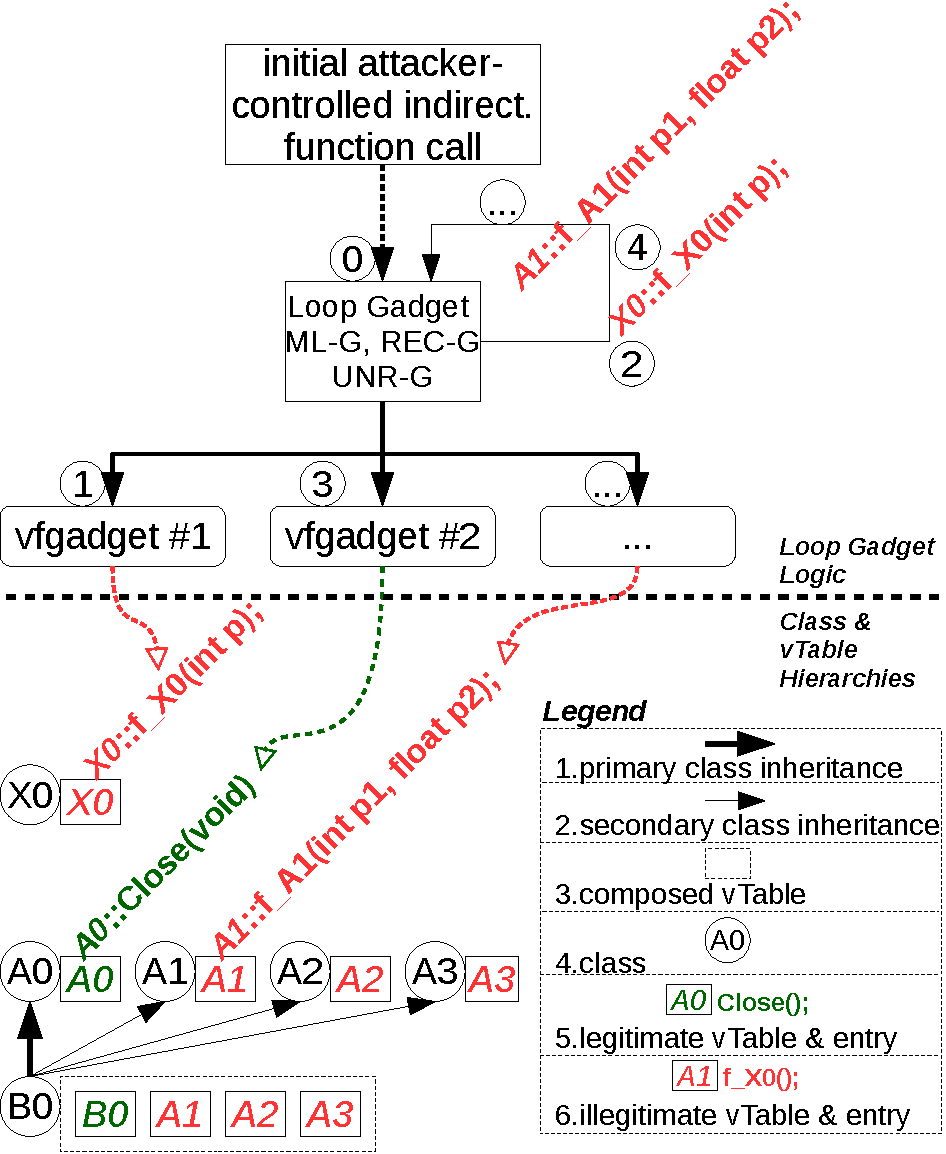
\includegraphics[width=1.3\textwidth]{figures/loop.pdf}
% % \end{minipage}
% % \caption{Code example used to illustrate how a COOP loop gadget works.}
% % \label{Code example used to illustrate how a COOP loop gadget works}
% % \end{figure}
% 
% %%%%%%%%%%%%%%%%%
% \begin{figure}[!t]
%    \centering
%    \setlength{\unitlength}{0.1\textwidth}
%    \begin{picture}(10,4)
%      \put(2.85,0){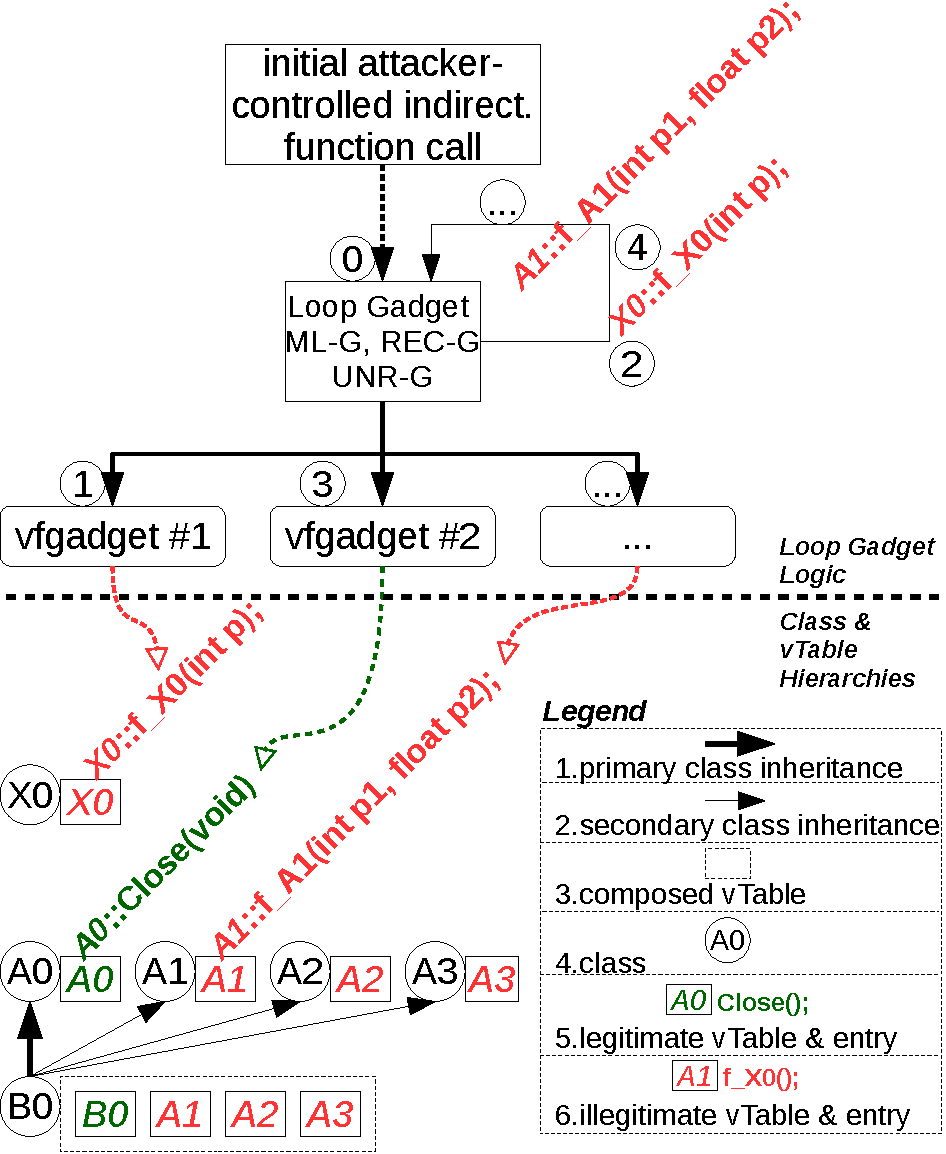
\includegraphics[width=.3\textwidth]{figures/loop.pdf}}
%      \put(0,2){\usebox{\firstlisting}}
%    \end{picture}
% \caption{Code presenting how a COOP loop gadget works.}
% \label{Code example used to illustrate how a COOP loop gadget works}
% \end{figure}


Figure~\ref{Code example used to illustrate how a COOP loop gadget works}
depicts a C++ code example where it is illustrated how a COOP loop gadget 
(\textit{i.e.,} ML-G, REC-G, UNR-G, see~\cite{crane:readactor++}) works.
The vfgadget \circled{1} can be exploited in several ways, see \textit{x), y) and z)} above.
The indirect callsite (Figure~\ref{Code example used to illustrate how a COOP loop gadget works} line 17) can be exploited 
to call by passing a varying number of parameters and types
on each object contained in the array a different
vTable entry contained in the:
\textit{1)} class hierarchy (overall, whole program),
\textit{2)} class hierarchy (partial, only legitimate for this callsite),
\textit{3)} vTable hierarchy (overall, whole program),
\textit{4)} vTable hierarchy (partial, only legitimate for this callsite),
\textit{5)} vTable hierarchy and/or class hierarchy (partial, only legitimate for this callsite), and
\textit{6)} vTable hierarchy and/or class hierarchy (overall, whole program).
There is no language semantics---such as cast checks---in C++ for vCall sites dispatch checking and as consequence
the loop gadget indicated in Figure~\ref{Code example used to illustrate how a COOP loop gadget works}
can basically call all around in the class and vTable hierarchy by not being constrained by any build in check during
runtime. The attacker corrupts an indirect function call, \circled{1}, 
next she invokes gadgets,  \circled{1} and \circled{3}, 
through the calls, \circled{2} and \circled{4}, contained in the loop. 
As it can be observed in Figure~\ref{Code example used to illustrate how a COOP loop gadget works} she 
can invoke from the same callsite legitimate functions residing in the vTable inheritance path
(\textit{i.e.,} this type of information is usually very hard to recuperate from executables)
for this particular callsite, indicated with green color vTable entries. 
However, a real COOP attack invokes illegitimate
vTable entries residing in the whole initial program hierarchy (or the extended one)
with less or no relationship to the initial callsite,
indicated with red color vTable entries.

\subsection{Checking Indirect Calls in Practice}
% \textbf{Checking Indirect Forward-Edge Calls in Practice.}
\label{C++ Indirect Calls in Practice}
To the best of our knowledge, there are only the IFCC/VTV~\cite{vtv:tice} tools (up to 8.7\% performance overhead) deployed in practice
which can be used to check legitimate from illegitimate indirect forward-edge calls during runtime.
vPointers are checked based on the class hierarchy. Furthermore, ShrinkWrap~\cite{haller:shrinkwrap} (to the best of our knowledge not deployed in practice)
is a tool which further reduces the legitimate vTbles ranges for a given indirect callsite
through precise analysis of the program class hierarchy and vTable hierarchy. 
Evaluation results show similar performance overhead but more precision w.r.t. to legitimate vTables entries per callsite.
We noticed by analyzing the previous research results that the overhead incurred by
these security checks can be very high due to the fact that for each callsite many range checks 
have to be performed during runtime. Therefore, despite its security benefit these types of
checks can not be applied in our opinion to high performance applications.

As alternative, there are other highly promising tools (also not deployed in practice) that can be used to mitigate 
some of the drawbacks of the previous tools. 
Bounov \textit{et al.}~\cite{bounov:interleaving} presented a tool ($\approx$ 1\% runtime overhead)
for indirect forward-edge callsite checking based on vTable layout interleaving. The tool has better performance
than VTV and better precision w.r.t. allowed vTables per indirect callsite. Its precision (selecting legitimate vTables for each callsite)
compared to ShrinkWrap is lower since it does not consider vTable inheritance paths.
vTrust~\cite{zhang:vtrust} (average runtime overhead 2.2\%) enforces two layers of defense (virtual function type enforcement and vTable pointer sanitization)
against vTable corruption, injection and reuse.
TypeArmor~\cite{veen:typearmor} ($\le$ than 3 \% runtime overhead) enforces an CFI policy based on runtime checking of caller/caller pairs based
on function parameter count matching (coarse grained, parameter types and more than six parameters can be used as well).
Important to notice is that there are no C++ language semantics which can be used to enforce type and 
parameter count matching for indirect call/callee pairs, this could be addresses with specifically intended language constructs in the future.

\subsection{Security Implications of Indirect Calls}
% \textbf{Security Implications of Forbidden Indirect Calls.}
\label{Security Implications of Forbidden Forward Indirect Calls}
The C++ language standard (12.7~\cite{iso:iecN3690}) does not specify
what happens when calling different vTable entries from an indirect callsite.
The standard says that we have a virtual function related undefined behavior when:
\textit{a virtual function call uses an explicit class member access and the object expression refers to the complete
object of x or one of that object’s base class subobjects but not x or one of its base class subobjects}.
As undefined behavior is not a clearly defined concept we argue that in order to be able to deal
with undefined behavior or  unspecified behavior related to virtual function calls one needs to know
how these languages dependent concepts are implemented inside the used compilers.

Forbidden forward-edge indirect calls are the result of a vPointer corruption.
A vPointer corruption is not a vulnerability but rather a capability which 
can be the result of a spatial or temporal memory corruption through: 
(1) bad-casting~\cite{byoungyoung:typecasting} of C++ objects, 
(2) buffer overflow in a buffer adjacent to a C++ object or a use-after-free condition~\cite{schuster:coop}.
A vPointer corruption can be exploited in several ways. A manipulated vPointer
can be exploited by pointing it in any existing or added program vTable entry 
or into a fake vTable which was added by an attacker. For example in case a vPointer
was corrupted than the attacker could highjack the control flow of the program 
and start a COOP attack~\cite{schuster:coop}.

vPointer corruptions are a real security threat which can be exploited if there 
is a memory corruption (\textit{e.g.,} buffer overflow) which is adjacent to
the C++ object or a use-after-free condition. As a consequence each corruption 
which can reach an object (\textit{e.g.,} bad object casts) is a potential exploit vector 
for a vPointer corruption. Interestingly to notice in this context is that through:
(1) memory layout analysis (through highly configurable compiler tool chains) of 
source code based locations which are highly prone to
memory corruptions such as declarations and uses of buffers, integers or pointer 
deallocations one can obtain the internal machine code layout representation.
(2) analysis of a code corruption which is adjacent (based on (1)) to a C++ object based on
application class hierarchy, the vTble hierarchy and each location in source code where an object
is declared and used (\textit{e.g.,} modern compiler tool chains can spill out this information for free), 
one can derive an analysis which can determine---up to a certain extent---if a memory corruption 
can influence (is adjacent) to a C++ object.

Finally, we notice that by building tools based on this two concepts (\textit{i.e.,} (1) and (2))
attackers (\textit{e.g.,} used to find new vulnerabilities) and for defenders which can 
harden the source code with checks only at the places which are most exposed 
to such vulnerabilities (\textit{i.e.,} we name this targeted security hardening).

\subsection{Imprecise Parameter-Count Policies}
% \textbf{Permissive Parameter-Count-Based Policies.}
\label{Too Permissive Parameter-Based Policies}
TypeArmor~\cite{veen:typearmor} is a tool that can enforce a CFI runtime policy for dispatching of call sites based only on
parameter count. The authors claim that their policy reports only an \textit{overestimation} for the parameters prepared by a call site
and \textit{underestimation} for the number of parameters consumed by the matching call targets. The authors claim that their technique is 
effective w.r.t. preventing COOP attacks. 

We do not agree with this claim and furthermore we believe that their call site vs. call target set enforcing policy is too permissive and thus many potential indirect forward edge based 
control flow transfers are possible. Consider the following example. In the best case for each call site preparing say $p=4 \in [1, 6]$ parameters their policy
could theoretically allow only the call targets which consume the same number as parameters as prepared, $c=4 \in [1, 6]$. Note that this does not hold due to 
the aforementioned call site overestimation and call target underestimation, thus all possible numerical mismatches are allowed by their policy as long as $p$ is 
greater or equal to $c$.

\begin{itemize}
\item TypeArmor \textit{ideally} would allow for a single call site a set of call targets containing maximum $117649$ possibilities if we 
consider the maximum value of provided parameters to be
$p=6$ due to $p \in [1, 6]$ possible provided parameters. Consider 7 C++ integer parameter types $t$:
$int$, $char$, $unsigned char$, $bool$, $long$, $unsigned long$,  and $short$. 
Thus we obtain $t^{p}=7^{6}=117649$ allowed call targets per call site if the TypeArmor is in place.
Note that for simplicity reasons we considered $t=7$ but in practice $t$ is even larger since there are many types of parameters in C++. 
The complete list of fundamental C++ types contains 20 types; not including data structures or object types.
Thus, all these data types would be ignored by TypeArmor. Also, note that all other call sites having more than 6 parameters 
would be not checked by TypeArmor as well.

\item TypeArmor \textit{actually} allows more than $t^{p}$ call targets per call site.
If we have $t=7$ integer types due to TypeArmors overestimation and underestimation we get for each call site an additional
number of call targets. Let $p=6$ than we get $c = 6x + 5y+ 4z + 3t + 2p + 1v$ where:
$x$ is the sum of all call targets consuming 6 parameters, 
$y$ is the sum of all call targets consuming 5 parameters 
and so on up to 0 parameters. Note that this holds since TypeArmor allows more parameters provided than consumed by the calltarget.
Than $c = 2100 = 600 + 500 + 400 + 300 + 200 + 100 \ iff \ x=y=z=t=p=v=100$. 
Note that $x=100$ is feasible under realistic conditions in large applications (\textit{i.e.,} Google Chrome, Firefox). 
Next $2100$ is added to $7^{6}$. 
Thus for a single call site providing $p=6$ parameters TypeArmor allows theoretically in 
total $7^{6} + 2100 = 1197496$ call targets for each callsite.
This holds for $p=5$ where we get $7^{5} + (1500 = 500 + 400 + 300 + 200 + 100) = \ 18307 \ iff \ x=y=z=t=p=v=100$ 
allowed call target per call site. Note that this holds for $p \in [1, 4]$ too.
\end{itemize}

Finally, TypeArmor is too permissive and as consequence we present 
\textsc{TypeShield} which deals with the variable type state explosion due to different parameter types by considering an 
approximation (\textit{i.e.,} alias analysis and thus type analysis in binaries is undecidable~\cite{alias:undecidable}) of 
parameter types based on register wideness. Consequently, the allowed call target set for each call site is drastically reduced.

\subsection{Real COOP Attack Example}
% \textbf{Real COOP Attack Example.}
\label{Running Example: CVE X}
%%second pic
\begin{figure}[h!]
    \centering
    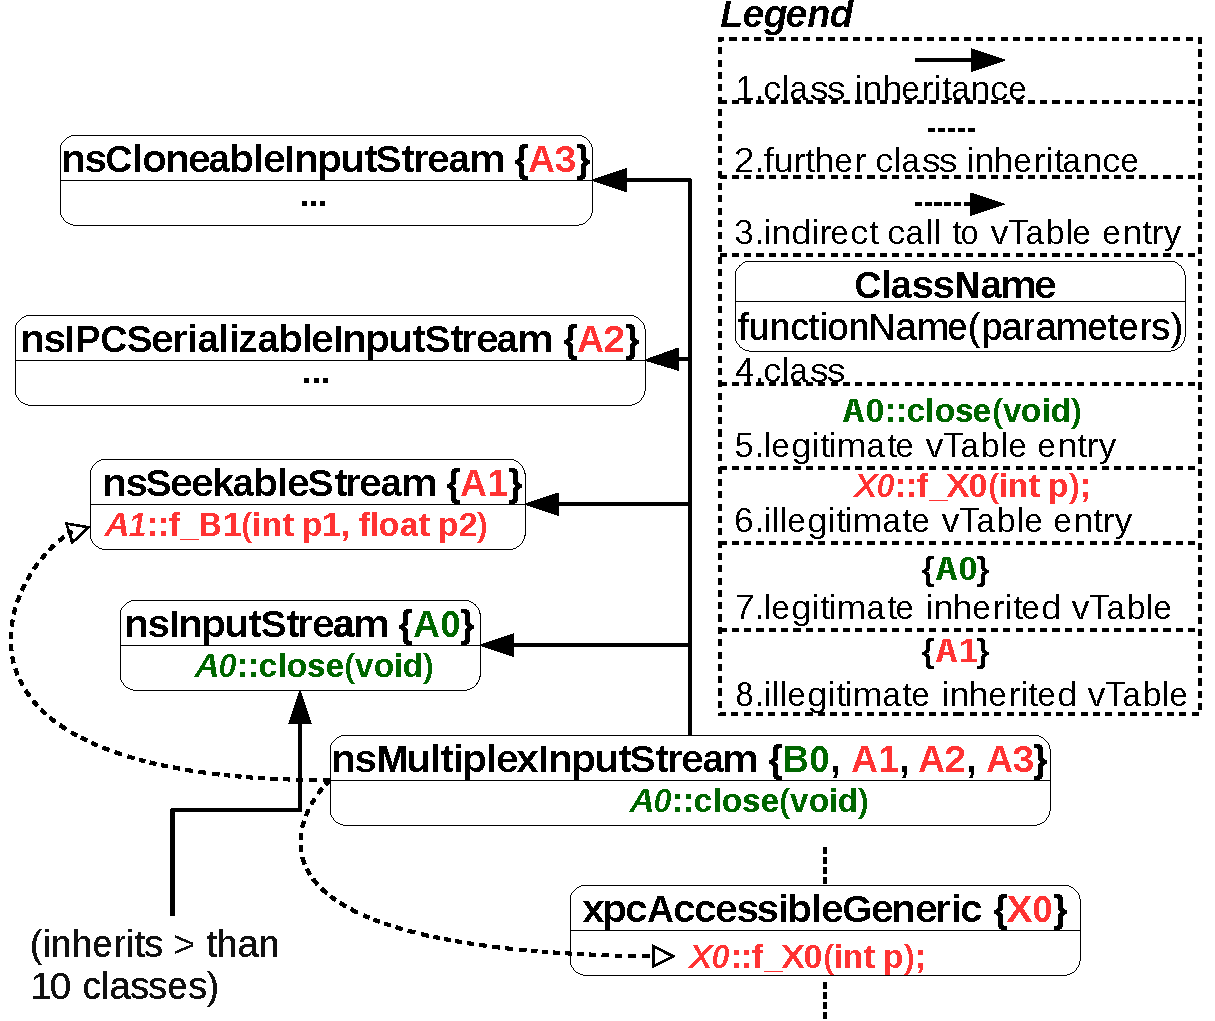
\includegraphics[width=0.47\textwidth]{figures/class_hierarchy.pdf}
\caption{Class inheritance hierarchy of the classes involved in the COOP attack against the Firefox browser. Red letters 
indicate forbidden vTble entries and green letters indicate allowed vTable entries for the given indirect callsite
contained in the main loop gadget.}
\label{Class exploit}
\end{figure}
The next COOP attack example depicted in Figure~\ref{Class exploit}
is a proof of concept exploit extracted from~\cite{schuster:coop} and used in order to perform 
a COOP attack on the Firefox browser. A buffer overflow bug was used in order to call 
into existing vTable entries by using a main loop gadget. 
The attack concludes with opening of an Unix shell. 
A real-world bug, CVE-2014-3176, was exploited by Crane \textit{et al.}~\cite{crane:readactor++}
in order to perform another COOP attack, on the Chromium browser. The details of the 
second attack are far to complex (\textit{i.e.,} involves not properly handled interaction of 
extensions, IPC, the sync API, and Google V8) and for this reason we briefly present the first 
documented COOP exploit on a Linux machine.

The C++ class \texttt{nsMultiplexInputStream} contains a main loop gadget inside the function 
\texttt{nsMultiplexInput-} \texttt{Stream::Close(void)} which is performing indirect calls by dispatching
indirect calls on the objects contained in the array. 
The objects contained in the array during normal execution are of type \texttt{nsInputStream} and each
of the objects will call the \texttt{Close(void)} function in order to close each of the previously opened streams.
For performing the COOP attack the attacker crafts a C++ program containing an array buffer holding 
six fake objects. Fake objects can call inside (and outside) the initial class and vTable hierarchies
with no constraints.
During the attack a buffer is created in order to hold the fake objects.
The crafted buffer will be used instead of the real code in order to call different functions
available in the program code. For example, the attacker calls a function contained in the class
\texttt{xpcAccessibleGeneric} which is not in the class hierarchy or vTable hierarchy
of the initially intended type of objects used inside the array.
Moreover, the header file of this class (\texttt{xpcAccessibleGeneric}) is not included in the 
class \texttt{nsMultiplexInputStream}.
In total six fake objects are used to call into functions residing in not related class hierarchies with varying 
number of parameters and return types. The final goal of this attack is to prepare the program memory such 
that a Unix shell can be opened at the end of this attack.

This example illustrates why detecting vPointer corruptions is not trivial for real-world applications.
As depicted in Figure~\ref{Class exploit} the class \texttt{nsInputStream} has 11 classes which inherit directly
or indirectly from this class. The classes \texttt{nsSeekableStream}, \texttt{nsIPCSerializableInputStream}
and \texttt{nsCloneableInputStream} provide additional inherited vTables which represent illegitimate calltargets
for the initial \texttt{nsInputStream} objects and legitimate calltargets for the six fake objects which were added during the attack.
Furthermore, declaration and usage of the objects can be wide spread in the source code. This makes
detection of the object types (\textit{i.e.,} base class), range of vTables (\textit{i.e.,} longest vTable inheritance path for a particular callsite)
and parameter types of the vTable entries (\textit{i.e.,} functions) in which it is allowed to call a 
trivial task for source code (\textit{i.e.,} current research work is mostly concerned with performance issues)
applications but a hard task in our opinion when one wants to apply similar security policies 
(\textit{e.g.,} which rely on parameter types of vTable entries) to executables.





